% compile with: lualatex -shell-escape filename.tex
\documentclass[tikz]{standalone}
\directlua{luatexbase.add_to_callback(
  "wrapup_run",
  function() os.execute("pdf2svg \jobname.pdf \jobname.svg") print("Converted to SVG.") end,
  "final callback to convert pdf file")}

\usetikzlibrary{positioning}

\begin{document}

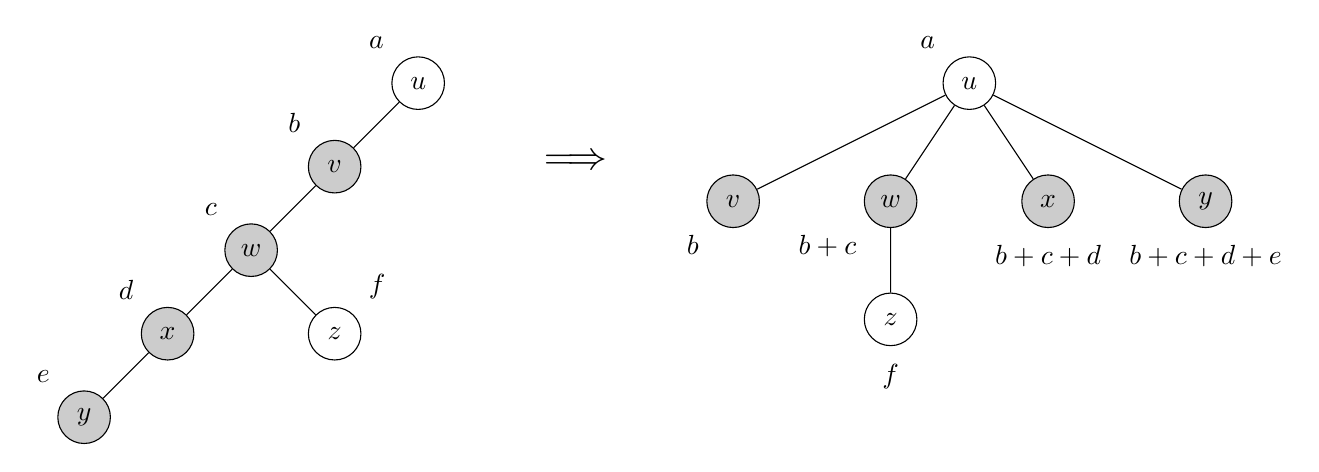
\begin{tikzpicture}[
  tree/.style={
    circle,
    draw,
    minimum size=19pt,
  },
  moved/.style={fill=black!20},
  ]
  \begin{scope}
    \node[tree] (u) {$u$}
    child[grow=south west] {node[tree, moved] (v) {$v$}
      child[grow=south west] {node[tree, moved] (w) {$w$}
        child[grow=south west] {node[tree, moved] (x) {$x$}
          child[grow=south west] {node[tree, moved] (y) {$y$}
          }
        }
        child[grow=south east] {node[tree] (z) {$z$}
        }
      }
    };

    \node[above left=1mm of u] {$a$};
    \node[above left=1mm of v] {$b$};
    \node[above left=1mm of w] {$c$};
    \node[above left=1mm of x] {$d$};
    \node[above left=1mm of y] {$e$};
    \node[above right=1mm of z] {$f$};
  \end{scope}

  \begin{scope}[xshift=2cm, yshift=-1cm]
    \node{\Large $\Longrightarrow$};
  \end{scope}

  \begin{scope}[
    xshift=7cm,
    level 1/.style={sibling distance=20mm},
    ]
    \node[tree] (u) {$u$}
    child[] {node[tree, moved] (v) {$v$}}
    child[] {node[tree, moved] (w) {$w$}
      child[] {node[tree] (z) {$z$}}
    }
    child[] {node[tree, moved] (x) {$x$}}
    child[] {node[tree, moved] (y) {$y$}};

    \node[above left=1mm of u] {$a$};
    \node[below left=1mm of v] {$b$};
    \node[below left=1mm of w] {$b + c$};
    \node[below=1mm of x] {$b + c + d$};
    \node[below=1mm of y] {$b + c + d + e$};
    \node[below=1mm of z] {$f$};
  \end{scope}
\end{tikzpicture}

\end{document}
